\epigraph{Any fool can write code that a computer can understand. Good
programmers write code that humans can understand}{Martin Fowler}

	Pentru orice sistem software vrem să fim în stare să verificăm/să evaluăm: 
	\begin{itemize}
	    \item calitatea sistemului, a codului scris, a design-ului
		\item test coverage  
		\item respectarea standardelor impuse 
		\item folosirea sau nu a  hack-urilor de limbaj.
	\end{itemize}
	Pentru a putea fi în stare să facem acest lucru avem nevoie de tool-uri pentru
analiză de programare.
Desigur, există nenumărate programe care fac acest lucru:
	  \begin{description}[labelindent=2cm]
	  \item[Wala IBM] {analiză de fluxului de data, analiză cu respect la context,
\ldots{} }
	  \item[FindBugs]  depistează erorile  din  codul sursă
	  \item[IntelliJ]   O platformă care implementează 100+ de analizatori pentru
 cod.
	  \item[SonarJ]  Monitorizarea performanței aplicației
	  \item[CodePro] {Platformă care integrează numeroase metrici pentru software
analysis. Implementat de LOOSE Group.}
	  \end{description}
         Toate aceste tool-uri nu sunt create să ruleze doar pe un anumit cod, 
ci pe o clasa întreagă de programe. Pentru acest lucru ele definesc un metamodel.
Un metamodel reprezintă elementele necesare descrieri unui model, e.g în cazul 
codului sursă metamodelul reprezintă gramatica limbajului.	În figura \ref{fig:metamodels} 
se poate observa că există trei clase A, B, C care sunt descrise fară probleme
de metamodelul Class. Tot în această figură se poate observa că metamodelul 
Class nu este singurul care poate descrie clasele A, C, ci și metamodelul
MyClassEntity poate face acest lucru. Însă cum am putea să le unim ?
Cum am putea să descriem aceste metamodele ? Pentru a putea face
toate aceste lucruri într-un mod uniform avem nevoie de un meta-metamodel. 
Un exemplu de astfel de meta-metamodel este prezentat și în figura
\ref{fig:metametamodel}. 


\begin{figure}
\scalebox{0.4}{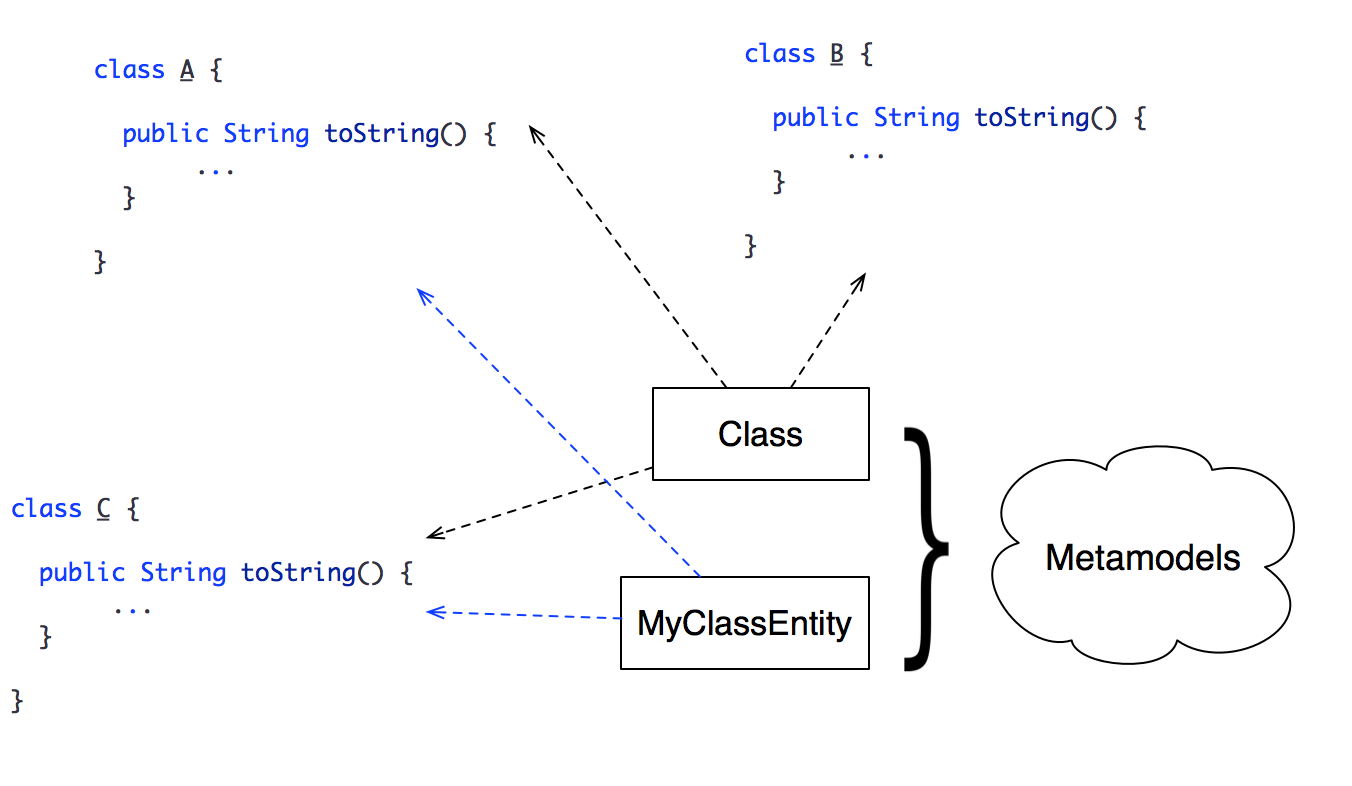
\includegraphics{img/Metamodels.png}}
\caption{Două metamodele diferite pentru același model}
\label{fig:metamodels}
\end{figure}
	
	Aceeași problemă apare și în cazul tool-urilor. Fiecare tool vine cu propriul
său metamodel care trebuie integrat în platformă. Noi ne dorim să creăm o
platformă care este ușor extensibilă și care permite integrarea cu ușurință a mai multor tool-uri, plugin-uri. 
Pentru acest lucru, însă, avem nevoie de un meta-metamodel.

\begin{figure}
\centering
\scalebox{0.4}{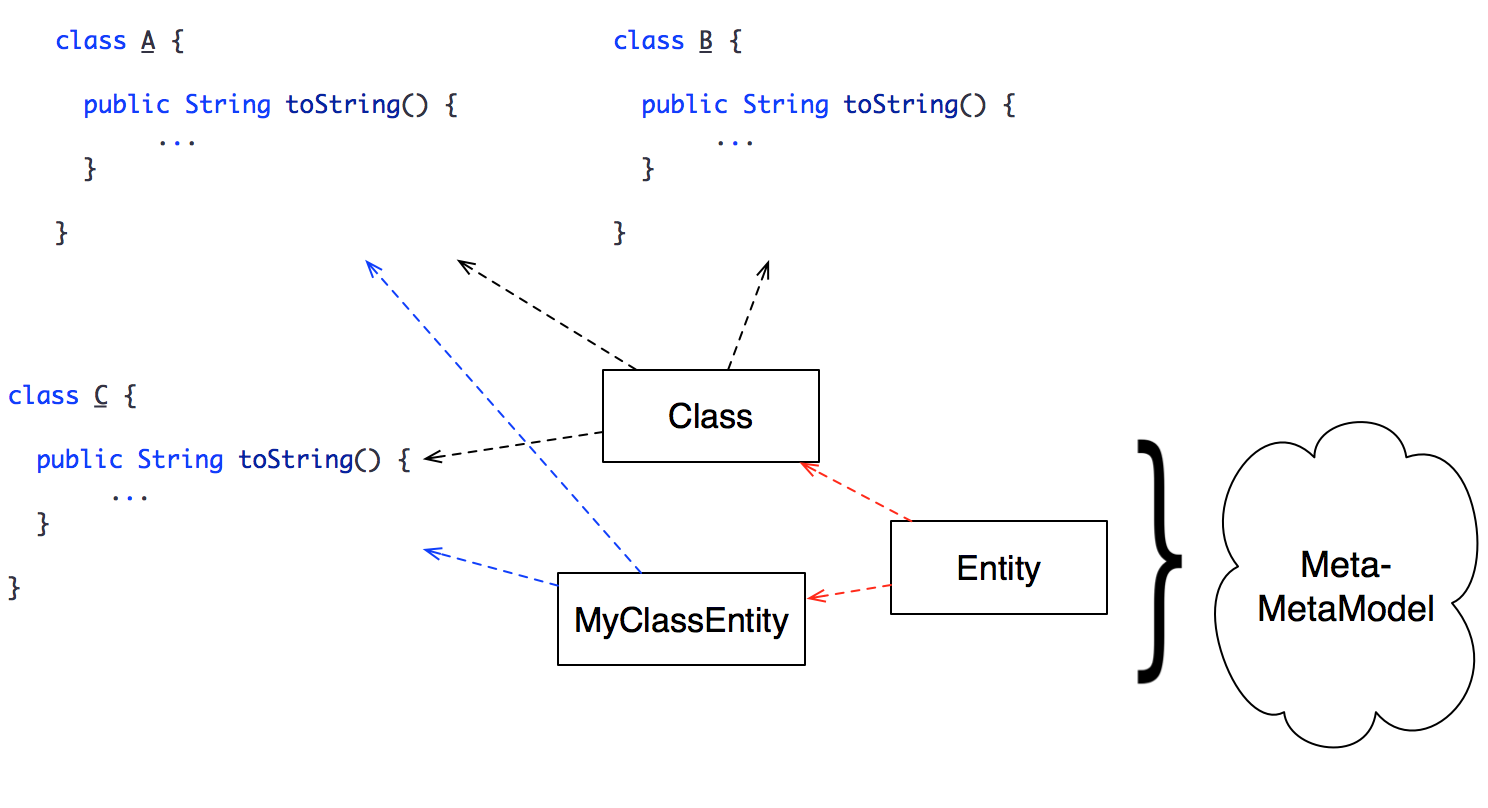
\includegraphics{img/Meta-Metamodel.png}}
\caption{Meta-Metamodele}
\label{fig:metametamodel}
\end{figure}	
	
	CodePro are  un  meta-metamodel care este ușor extensibil. 
Este foar ușor de adăugat o nou metrică: trebuie extinsă clasa PropertyComputer
așa cum face și clasa CycloAVG în figura \ref{fig:cycloAVG}. 

\begin{figure}
\scalebox{0.4}{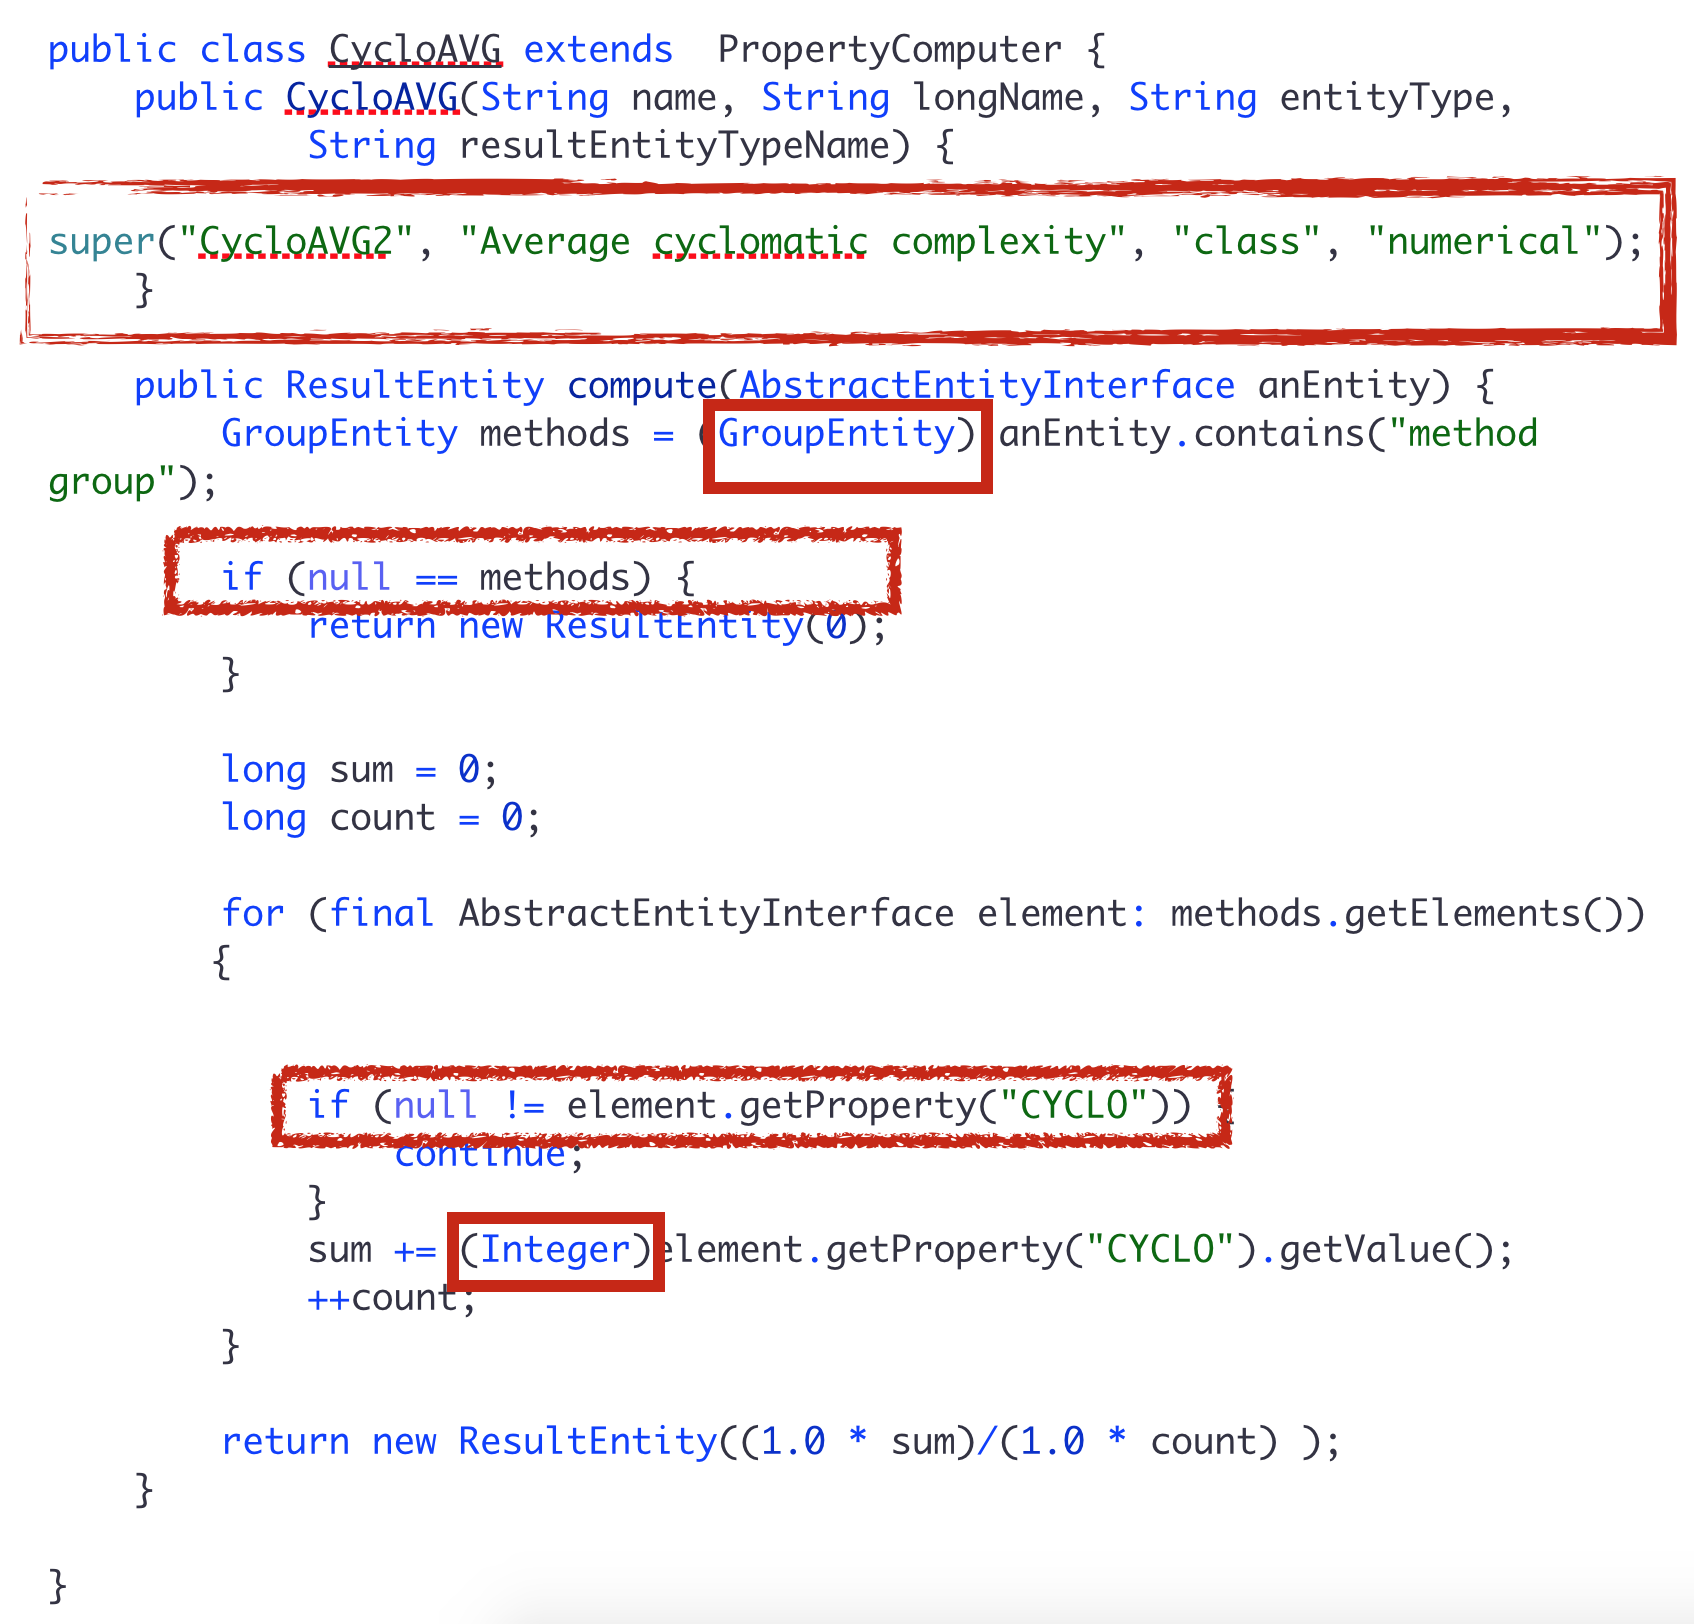
\includegraphics{img/cycloAVG.png}}
\caption{CycloAVG implementat în CodePro}
\label{fig:cycloAVG}
\end{figure}

Tot în acestă
figură se pot observa marcate cu roșu anumite probleme de design ce apar
datorită arhitecturii:
	\begin{description}[labelindent=2cm]
		\item[constante \enquote{magice}] {Se poate observa în constructorul clasei
		faptul că metrica CycloAVG se înregistrează prin numele \enquote{CycloAVG}. Însă ce se
întămplă dacă mai există o metrică cu acest nume ? Ce se întămplă cu metricele care
depind de noi dacă metrica noastră își schimbă numele ?}
		\item[generalizare] {CycloAVG își propune să calculeze o valoare pentru clasă
însă funcția compute primește ca parametru un AbstractEntity. Ce se întâmplă
dacă acest entity este defapt o metodă sau pachet ?}
	\end{description}
	Orice eroare datorată problemelor menționate mai sus poate fi descoperită doar
la runtime. Astfel noi am reușit să devenim dynamically typed într-un limbaj
statically typed. Lucru ce dăunează grav întreținerii și dezvoltării platformei.
	

	Noi am dori să scriem codul ca în figura \ref{fig:cycloAVGXCore}. Se poate
observa clar faptul că CycloAVG procesează un ClassEntity și în același timp sunt clare 
toate dependințele acestei metrici. Cel mai important lucru de observat este
faptul că am devenit din nou statically typed, păstrând în același timp ușurința
de a extinde și integra alte elemente.

\begin{figure}
\scalebox{0.7}{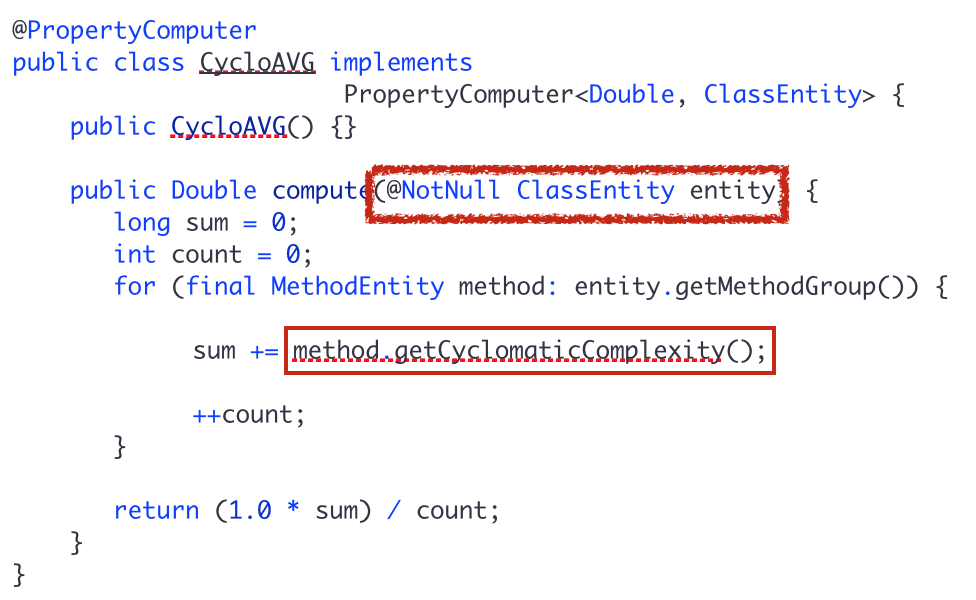
\includegraphics{img/cycloAVGXCore.png}}
\caption{CycloAVG implementat în XCore}
\label{fig:cycloAVGXCore}
\end{figure}

	XCore permite aceste lucruri prin reimplementarea meta-metamodelului din
CodePro. Meta-Metamodelul a fost implementat prin folosirea de adnotări.
Adnotări sunt elemente  Java prin care se poate asocia unuei clase,
metode, tip, \ldots{} etc, metainformație. În figura \ref{fig:cycloAVGXCore} se
poate observa că @PropertyComputer adontează clasa CycloAVG. Penru a putea
prelucra toate aceste metainformații avem nevoie de un procesor de adnotări. Un
procesor de adnotări este un plugin pentru compilator care atașează o semantică
pentru unul sau mai mutle adnotări. 

	Tot în figura \ref{fig:cycloAVGXCore} se poate observa folosirea unor
interfețe pentru a asigură consitența tipurilor și pentru a specifica
metamodelul necesar pentru metrica pe care o implementăm. În momentul când
compilăm proiectul, procesorul de adnotări a lui XCore va fi invocat. Acesta va
prelucra toate clasele adnotate și va genera codul necesar pentru metamodel
metricilor implementate.

	Acest tool este destul de greu de evaluat întrucât este dependent de
utilizator.  Pentru a îl putea evalua am reimplementat InsiderView, construind
XCoreView. InsiderView este un plugin pentru eclipse dezvoltat deasupra lui
CodePro și care face accesibilă platforma CodePro utilizatorilor Eclipse.
	
	În tabelul \ref{table:aggregated} se poate observa faptul că am reușit să
eliminăm complet toate constante \enquote{magice} și cast-urile care sunt
responsabile, cel puțin parțial, pentru problemele meționate la început. În
același timp aș dori să observați că numarul de linii de cod a rămas aproximativ
același, iar complexitatea generală a codului a scăzut. Astfel putem afirma că
tool-ul nostru a reușit cu succes să transforme toate plugin-urile din dynamic
typed în statically typed păstrând toate proprietățiile de exentesabilitate și
integrabilitate.
	
	

\begin{table}[h]
\centering
\caption{Agregarea valorilor pentru comparare. Cele mai importante valori
au fost colorate.}
\label{table:aggregated}
\resizebox{\textwidth}{!}{%
	\begin{tabular}{@{}ccccc@{}}
	\toprule
	 & Number of Lines & Cyclomatic Complexity & Number of Casts & Number of Magic Strings \\ \midrule
	Avg CodePro & \cellcolor[HTML]{32CB00}34.153 & \cellcolor[HTML]{F8FF00}4.307 & 1.796 & 2.230 \\
	Avg XCoreView & \cellcolor[HTML]{32CB00}31.384 & \cellcolor[HTML]{F8FF00}2.384 & 0 & 0 \\
	Sum CodePro & 444 & 56 & \cellcolor[HTML]{FD6864}23 & \cellcolor[HTML]{FD6864}29 \\
	Sum XCoreView & 408 & 31 & \cellcolor[HTML]{FD6864}0 & \cellcolor[HTML]{FD6864}0
	\end{tabular}
}
\end{table}		

	
		
	
 

